\chapter{Conclusiones}

Para finalizar este trabajo se van a resumir, en este Capítulo, las conclusiones extraídas para los objetivos planteados al inicio del proyecto, así como aquellas ideas que se pueden extraer del uso de las herramientas desarrolladas durante el caso de uso práctico.

Se puede afirmar que se han cumplido los objetivos propuestos dentro del plan establecido: se ha recopilado y analizado la información necesaria para desarrollar las cuestiones a discutir y se han llevado a la práctica estas ideas por medio de un caso práctico de uso. Además, como trabajo extra, se ha diseñado un framework para generar imágenes portables de shells personalizadas y se ha hecho una propuesta de aplicación de estas imágenes para docencia universitaria.

En esencia, el objetivo que se planteó era discernir qué puede aportar Wazuh al hacking ético y viceversa. Además de analizar las posibles interacciones entre estos dos ámbitos y desarrollar software para favorecer dichas interacciones.

Por un lado, se ha analizado cómo Wazuh puede ser un complemento a la hora de recopilar información de interés para los hackers éticos. Se ha desarrollado un módulo que permite integrar la ejecución de comandos en la app de Wazuh, almacenando su salida y sus metadatos, de forma que podamos clasificar los comandos ejecutados según ciertos criterios en función de su nivel de importancia, el tipo de evento que generan (reconocimiento, escalado de privilegios, análisis de vulnerabilidades, etc...) u otros criterios.

Por otro lado, en el caso de uso practico ha quedado claro que \textbf{Wazuh no es capaz de detectar cualquier ataque posible con una configuración por defecto}, de hecho, hace falta pensar bien cómo se quiere tratar de detectar cada tipo de ataque. Es por ello, que hacer tests de penetración de sistemas sobre una máquina con Wazuh instalado \textbf{puede ser una muy buena forma de evaluar el rendimiento de Wazuh y encontrar formas de mejorar el software o su configuración específica en un sistema}.

Por tanto, podemos concluir que, efectivamente, Wazuh puede ser una buena herramienta para complementar las labores de hackers éticos y, del mismo modo, actividades como los tests de penetración o los Bug Bounties pueden servir para \textbf{evaluar el rendimiento de Wazuh en un entorno} (como se ha demostrado en el caso práctico), pudiendo un hacker ético \textbf{encontrar puntos sin analizar por Wazuh} que se pueden solucionar por medio de configuraciones extra, plugins, integraciones con otros softwares,... abriendo un camino con infinidad de posibilidades.

Como parte del trabajo se ha desarrollado un framework para generar imágenes portables de consolas de comandos basadas en Xonsh, a las que se puede añadir configuraciones específicas, herramientas y dependencias adicionales, además de plugins para extender la funcionalidad de Xonsh. Estas imágenes se pueden cargar en XXH de forma que sean utilizadas cuando se establezca una sesión SSH con un host remoto, permitiendo así integrar las herramientas y configuraciones que se pudieran necesitar (por ejemplo, como parte de una auditoría de ciberseguridad) también en los hosts remotos a los que se accede. Además, se ha demostrado que este framework puede ser utilizado en otros ámbitos además del de la ciberseguridad y se ha hecho una propuesta de aplicación del mismo en el ámbito docente en una asignatura del Grado de ingeniería informática de la Universidad de Granada.

Este es un \textbf{proyecto de código abierto} por lo que todo el trabajo está disponible y abierto para posibles futuros proyectos relacionados, para los cuales también se han hecho algunas propuestas de posibles trabajos futuros: plugins, configuraciones o recopilaciones de dependencias que podría ser interesante explorar. Este framework desarrollado no formaba parte de los objetivos iniciales pero se ha concluido que podía explotarse la idea y crear, junto con el resto del trabajo, una herramienta que pudiera ser utilizada con distintos fines (y no solo para la integración con Wazuh). 

Entre las ventajas de utilizar el framework desarrollado se destaca la posibilidad de homogeneizar el acceso a las máquinas, proporcionando una shell que se puede ejecutar en cualquier sistema operativo compatible con Python (incluso si no tiene Python instalado o tiene una versión muy vieja, puesto que la imagen generada incluye un Python embebido), incluyendo Windows, Solaris, HPUX, AIX, etc..., de forma que la experiencia de usuario sea \textbf{la misma independientemente del sistema operativo}.

En total, se han creado (o clonado y posteriormente modificado) \textbf{8 repositorios públicos} como parte de la organización creada para albergar todo el contenido desarrollado durante el proyecto. En total se han hecho cerca de 100 commits con más de \textbf{258435} líneas de código. 

Además, durante el desarrollo del trabajo \textbf{se ha colaborado activamente con dos proyectos open-source}, xonsh y xxh, se han abierto más de 15 issues varios pull request en estos y otros repositorios secundarios.

\begin{figure}[!hbt]
  \centering
  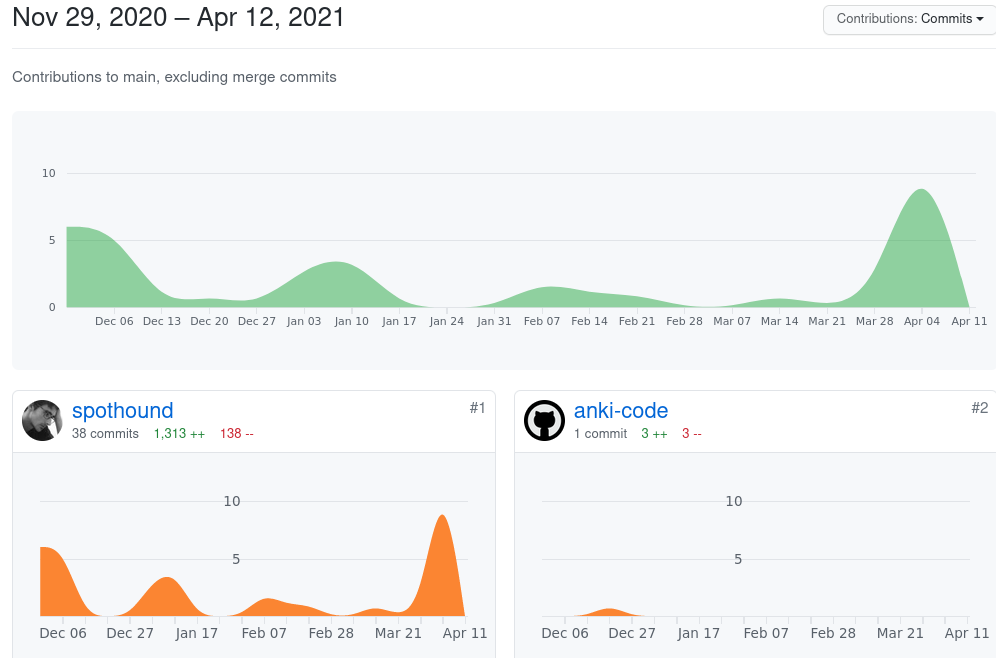
\includegraphics[width=\textwidth]{imagenes/github_activity.png}
  \caption{Visualización de la actividad del proyecto principal en github a lo largo del año en que se ha desarrollado el trabajo. Se puede apreciar que el proyecto incluso tiene una pequeña colaboración externa del \textbf{autor de xxh}. Aunque el número de commits o líneas de código no es muy elevado, se puede ver como el proyecto ha tenido actividad a lo largo de todo el año.}
  \label{githubactivity}
\end{figure}


Cabe destacar que \textbf{el autor de uno de estos proyectos se ha involucrado con el trabajo} creando algunas \textit{issues} con sugerencias para mejorar el proyecto e incluso abriendo un pull request (ver Figura \ref{githubactivity}).

En resumen, a lo largo del proyecto se han planteado una serie de hipótesis y experimentos para refutarlas que han sido llevados a cabo sin problema, se ha colaborado con proyectos open-source y se ha aportado a la comunidad creando una herramienta libre que además, se ha propuesto para ser utilizada en la docencia en la Universidad de Granada. 

Se ha cumplido el objetivo principal de analizar la relación entre Wazuh y el Hacking ético y se ha concluido que existen multitud de posibilidades para enlazar estos dos conceptos y sacar partido de su relación.

